% !TeX root = ../main.tex

\section{Verwendung}

Im folgenden Abschnitt wird ein Beispiel erläutert, bei dem die meisten Funktionalitäten des Projektes getestet werden können.

% TODO: Schachfeldgröße überprüfen!
Zunächst muss ein Schachbrett bereitgestellt werden, bei dem ein Feld jeweils \mbox{$7\times7$~cm} groß ist. Somit wird garantiert, dass sich die Dezibots komfortabel bewegen und rotieren können. Auf dem Dezibot $D$, welcher eine Schachfigur simulieren soll, muss das \texttt{examples/""showcase/""embedded\_""chess\_""piece.ino} Programm $P_D$ installiert werden. Dort können die zu simulierende Figur, die auszuführenden Züge sowie weitere Kalibrierungsoptionen eingestellt werden.

Ein weiterer Dezibot muss als \emph{Beacon} $B$ agieren. Dieser sendet ein Infrarot"=Signal aus, um die Rotation eines Dezibots zu regeln (vgl. \autoref{sec:movement-ir}). Dafür muss auf diesem \texttt{examples/""showcase/""beacon.ino} $P_B$ installiert werden.

Wie in \autoref{fig:usage} angedeutet ist, muss $B$ außerhalb des Schachbretts platziert und ungefähr in die Mitte des Schachbretts ausgerichtet werden. $D$ muss auf jenem Feld platziert werden, welches in $P_D$ festgelegt wurde. Eine weiße Figur muss dabei in Richtung Norden zeigen, eine schwarze in Richtung Süden. Die Richtungen sind aus dem in \autoref{fig:usage} dargestellten Kompass zu entnehmen.

\begin{figure}[h]
    \centering
    \begin{subfigure}[c]{0.49\textwidth}
        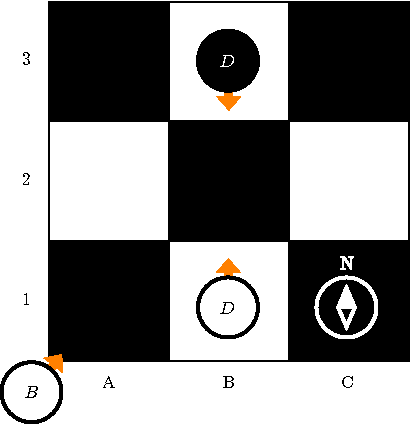
\includegraphics[width=\textwidth]{../assets/usage.drawio.pdf}
    \end{subfigure}
    \hspace{0.5em}
    \begin{subfigure}[c]{0.47\textwidth}
        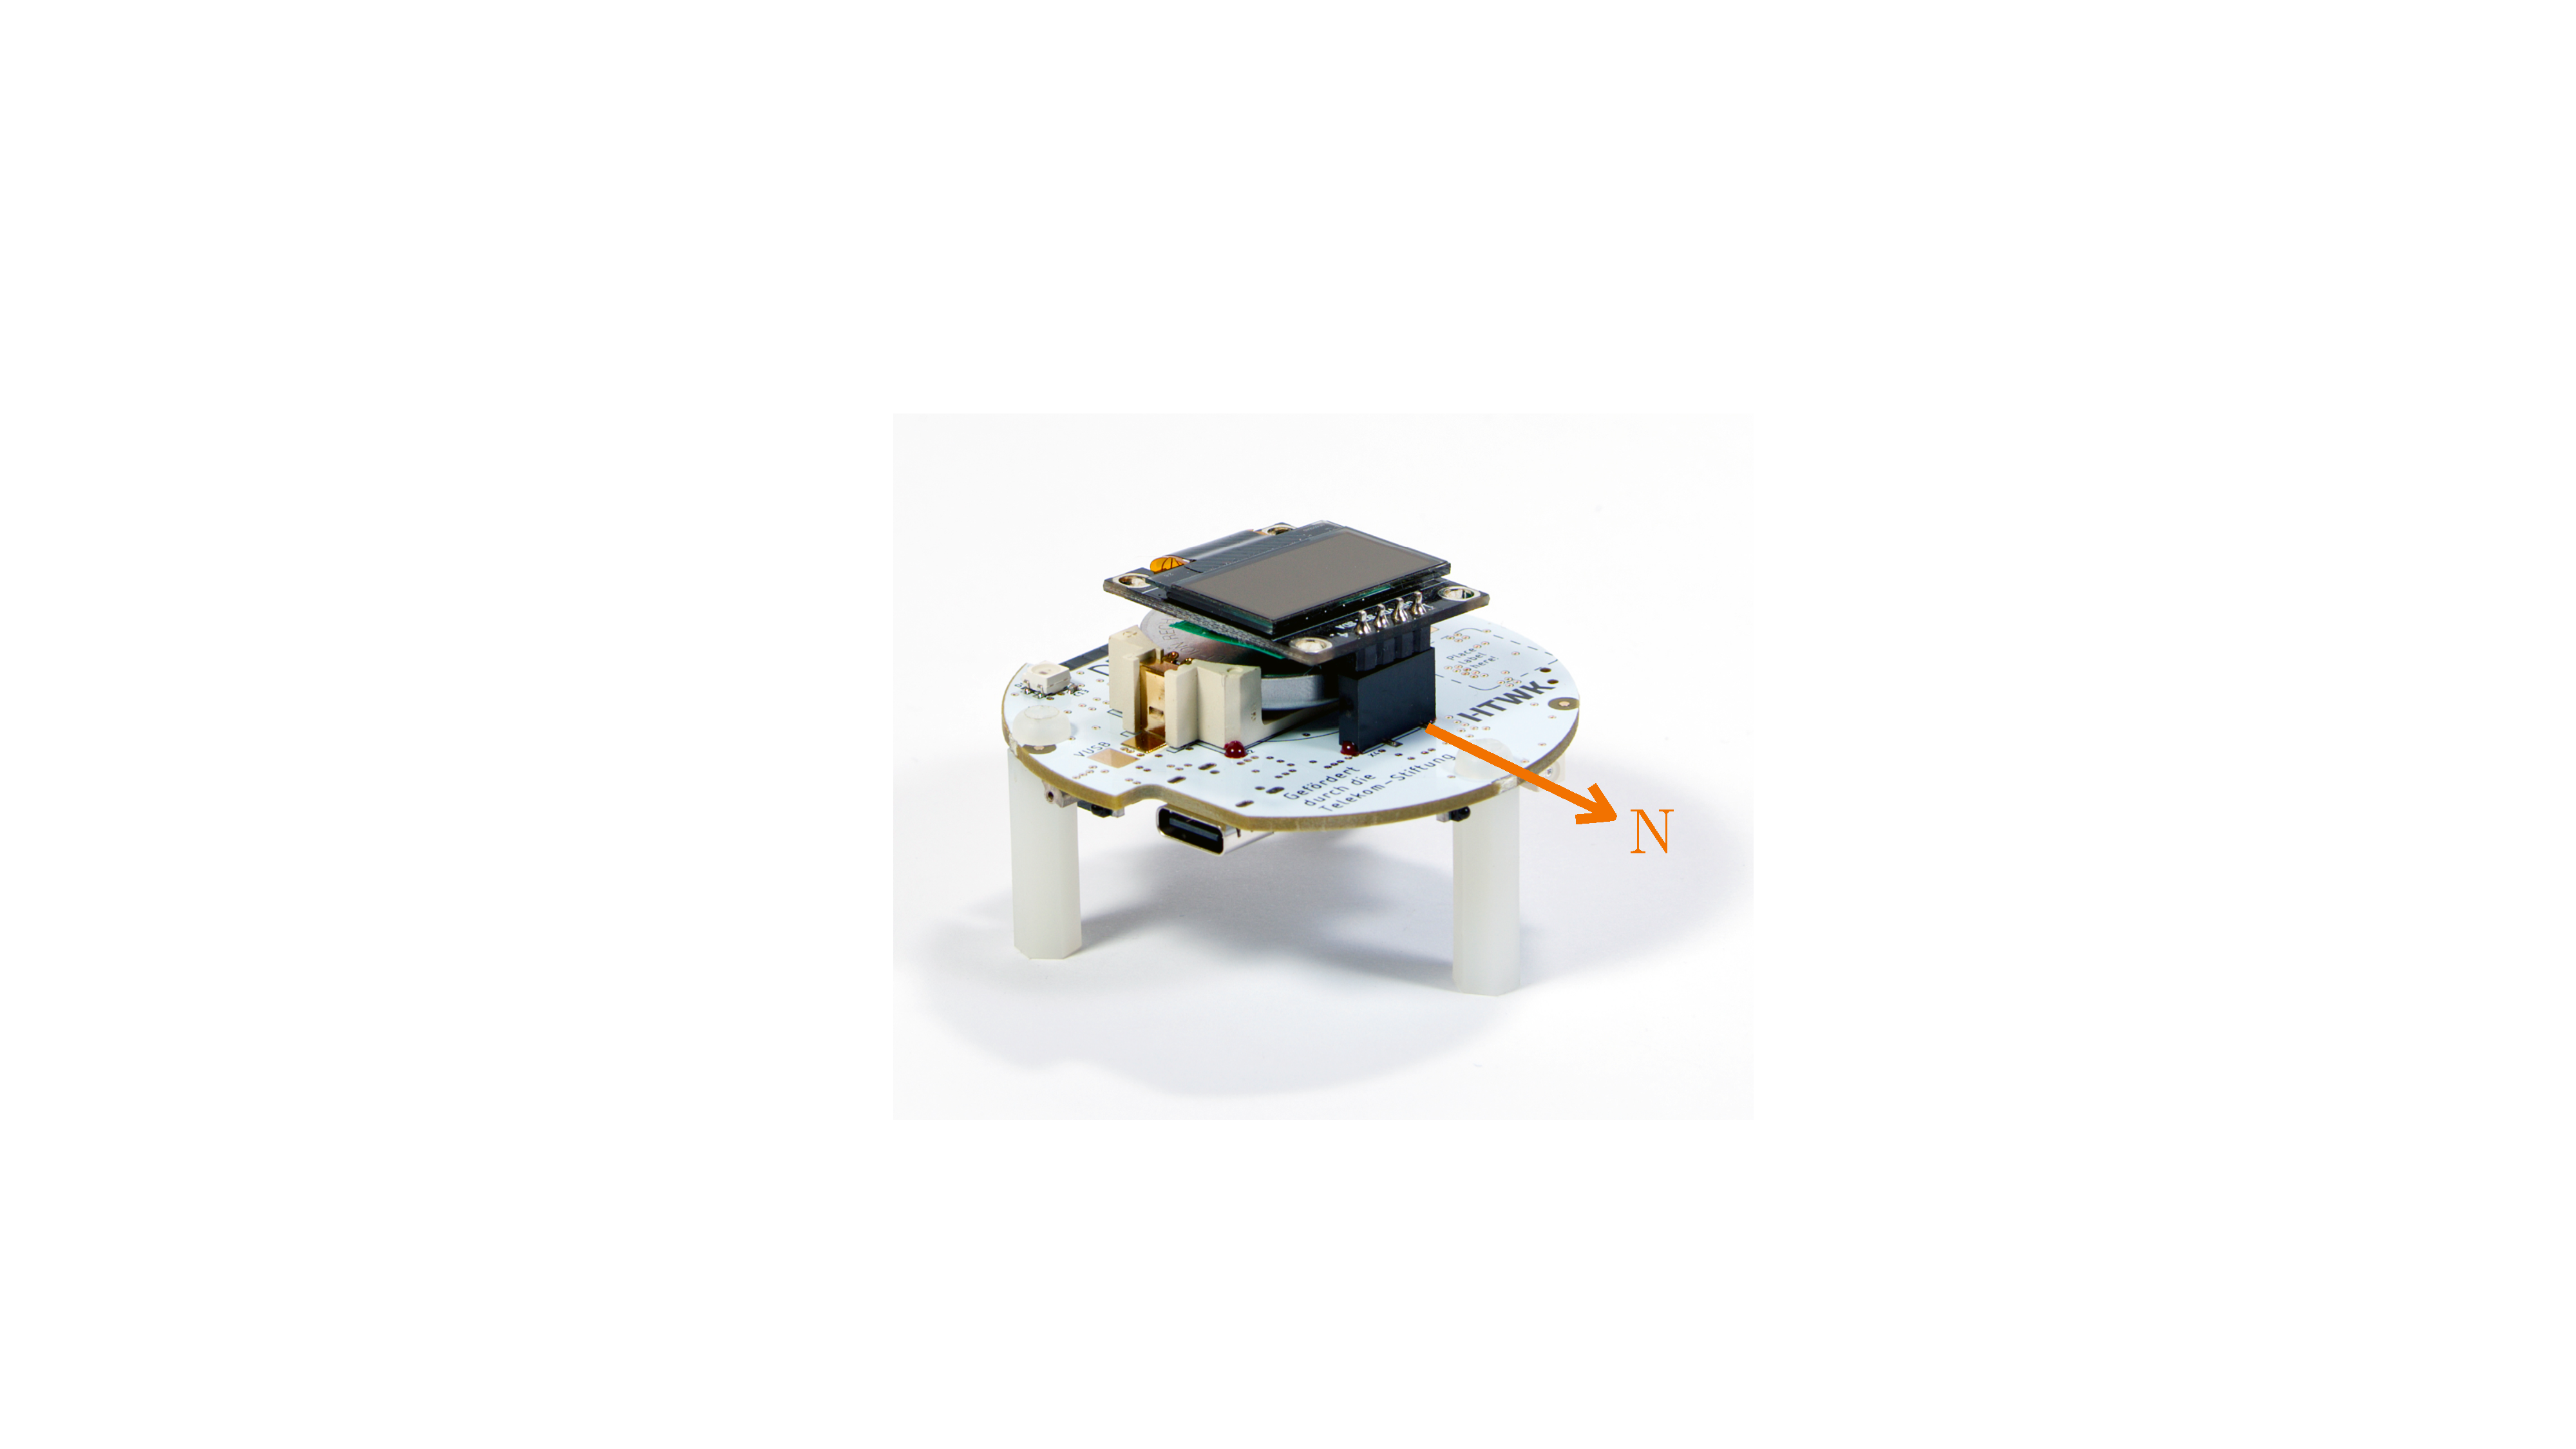
\includegraphics[width=\textwidth]{../assets/dezibot_total_view_north.png}
    \end{subfigure}
    \caption{Links: Ausschnitt eines Schachbretts, auf dem zwei Dezibots ($D$) dargestellt sind, welche eine weiße bzw. schwarze Figur simulieren. Unten links ist ein dritter Dezibot dargestellt, welcher als Beacon ($B$) agiert. In orange sind die Ausrichtungen der jeweiligen Dezibots angedeutet, welche rechts mit einem physikalischen Dezibot verdeutlicht wird. Dabei zeigt der rote Pfeil in Richtung Norden (Verwendung des speziell entworfenen 3D-gedruckten Modells~\cite[vgl.][]{felttipDezibotAlignmentPointer2025})}.
    \label{fig:usage}
\end{figure}

% TODO: initiale Kalibrierung notwendig?
